\documentclass[tikz,multi]{standalone}
\usepackage{color}
\usepackage{xcolor} 
\usepackage{tikz}
\usetikzlibrary{calc,backgrounds,fit,graphs,arrows,shapes,positioning,decorations.pathmorphing} 
 
%----------------------------------------------------------------------------------------------------------------
% Colors
%----------------------------------------------------------------------------------------------------------------
\definecolor{Orange}{RGB}{255,102,0}
\definecolor{DarkBlue}{RGB}{31,119,180}
\definecolor{DarkGreen}{RGB}{0,128,0}
\definecolor{Lime}{RGB}{188,189,34}
\definecolor{Purple}{RGB}{148,103,189}
\definecolor{Turquoise}{RGB}{23,190,207}
\definecolor{Magenta}{RGB}{227,119,194}
 
\begin{document}

%----------------------------------------------------------------------------------------------------------------
% Complete neuron-glia network scheme
%----------------------------------------------------------------------------------------------------------------
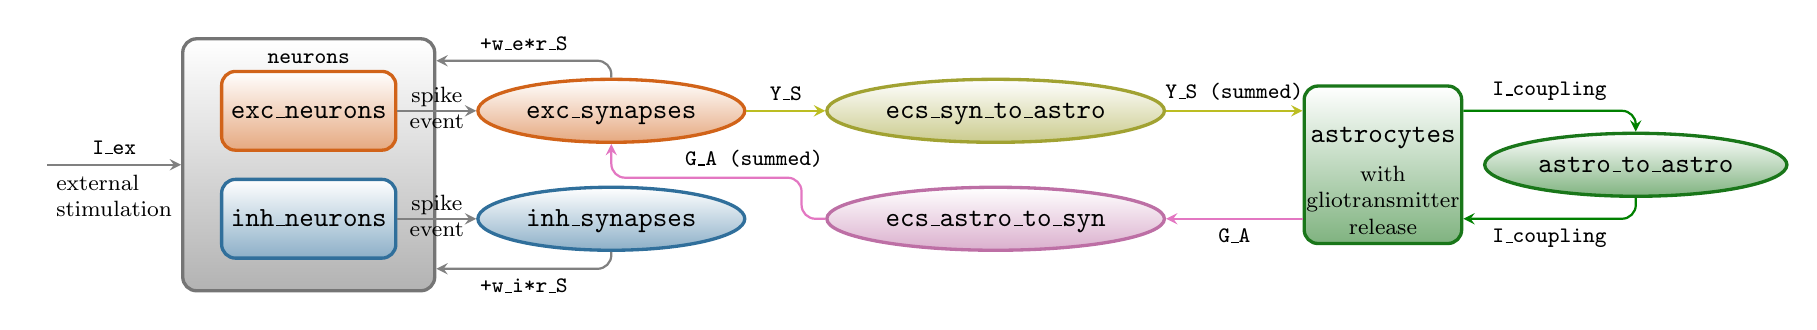
\begin{tikzpicture} [>=stealth, black!50, text=black, thick,rounded corners=5pt,
	   every new ->/.style = {shorten >=1pt},
	   every node/.style={font=\footnotesize},
	   neurongroup/.style 2 args = {rectangle, minimum size=#1, 
	                                very thick, draw=#2!80!black!90, top color=white,
                                    bottom color=#2!80!black!50,
                                    font=\ttfamily, text height=1.5ex,text depth=.25ex},
       synapsegroup/.style 2 args = {ellipse, minimum size=#1, 
	                                very thick, draw=#2!80!black!90, top color=white,
                                    bottom color=#2!80!black!50,
                                    font=\ttfamily, text height=1.5ex,text depth=.25ex}]
	%% Neurons
	\node [neurongroup={10mm}{Orange}] (exc) {exc\_neurons};
	\node [neurongroup={10mm}{DarkBlue},below=8.5mm of exc.center] (inh) {inh\_neurons};
	\begin{scope}[on background layer]
		\node [neurongroup={32mm}{gray},fit=(exc) (inh),
		       label={[shift={(0ex,-3ex)}]north:{\texttt{neurons}}}] (neurons) {};
	\end{scope}
	
	%% Reference node for external input
	\node [draw=none,left=1.7cm of neurons.west] (iex) {};
	
	%% Synapses
	\node [synapsegroup={8mm}{Orange},right = 1cm of exc.east] (exc_syn) {exc\_synapses};
	\node [synapsegroup={8mm}{DarkBlue},right = 1cm of inh.east] (inh_syn) {inh\_synapses};
	
	%% Extracellular space
	\node [synapsegroup={8mm}{Lime},right = 1cm of exc_syn.east] (ecs_s2a) {ecs\_syn\_to\_astro};
	\node [synapsegroup={8mm}{Magenta},right = 1cm of inh_syn.east] (ecs_a2s) {ecs\_astro\_to\_syn};

	%% Astrocytes
	\node [neurongroup={20mm}{DarkGreen},right = 11cm of neurons.east,
	       label={[shift={(0ex,2.5ex)},text height=1.5ex,text depth=.25ex,align=center]center:{\normalsize\texttt{astrocytes}}}] (astro) {};
	\node [below=-0.75ex,align=center] at (astro.center) {with\\gliotransmitter\\release};
	
	%% Gap junctions
	\node [synapsegroup={8mm}{DarkGreen},right = 0.25cm of astro.east] (gjc) {astro\_to\_astro};

	%% Simple paths
	\draw[->] (iex) -- (neurons.west)
			  node[above,align=center,midway] {\texttt{I\_ex}}
	          node[below,align=left,midway] {external\\stimulation};
	\draw[->] (exc) -- (exc_syn)
			  node[above=-0.5ex,align=center,midway] {spike} node[below=-0.5ex,align=center,midway] {event};
	\draw[->] (inh) -- (inh_syn)
	          node[above=-0.5ex,align=center,midway] {spike} node[below=-0.5ex,align=center,midway] {event};
	\path (exc_syn) edge[->,Lime,text=black] node[above,align=center,midway](ys) {\texttt{Y\_S}} (ecs_s2a);
	\path let \p1=(ecs_s2a.east),\p2=(astro.west) in (ecs_s2a) edge[->,Lime,text=black] node[above,align=center,midway] {\texttt{Y\_S (summed)}} (\x2,\y1);
	\path let \p1=(astro.west),\p2=(ecs_a2s.east) in (\x1,\y2) edge[->,Magenta,text=black] node[below,align=center,midway] {\texttt{G\_A}}(ecs_a2s);
	%% Complex paths
	\draw[->] let \p1=(neurons.north east) in (exc_syn.north) |- (\x1,\y1-3mm)
	          node[above,align=center,near end] {\texttt{+w\_e*r\_S}};
	\draw[->] let \p1=(neurons.south east) in (inh_syn.south) |- (\x1,\y1+3mm)
	          node[below,align=center,near end] {\texttt{+w\_i*r\_S}};
	\draw[->,DarkGreen,text=black] let \p1=(astro.east), \p2=(ecs_s2a.east) in (\x1,\y2) -| (gjc.north) 
	          node[above,align=center,near start] {\texttt{I\_coupling}};
	\draw[->,DarkGreen,text=black] let \p1=(astro.east), \p2=(ecs_a2s.east) in (gjc.south) |- (\x1,\y2)
	          node[below,align=center,near end] {\texttt{I\_coupling}};
	\draw[->,Magenta,text=black] let \p1=(ecs_a2s.west),\p2=(exc_syn.south),\p3=(ys.south),\p4=(inh_syn.north) in (\p1) -- (\x3 + 2mm,\y1) -- (\x3 + 2mm,\y4+1mm) -- coordinate(lbl1) (0.5*\x3 + 0.5*\x2 + 1mm,\y4+1mm) -- (\x2,\y4+1mm) -- (\x2,\y2);
	\node[above,align=center] at (lbl1) {\texttt{G\_A (summed)}};          
\end{tikzpicture}

%----------------------------------------------------------------------------------------------------------------
% Simple neuronal network (COBA)
%----------------------------------------------------------------------------------------------------------------
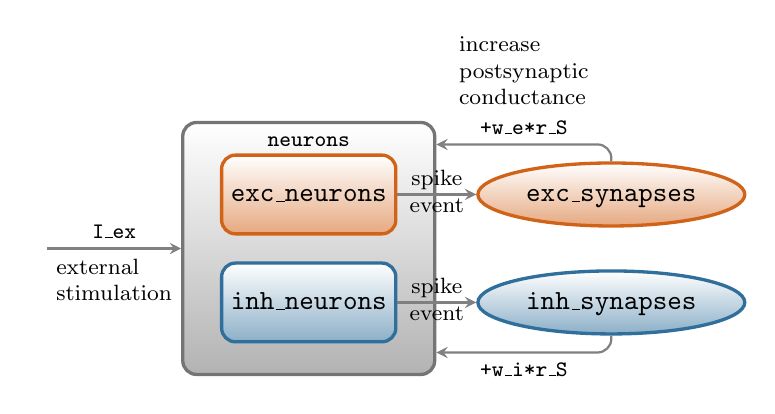
\begin{tikzpicture} [>=stealth, black!50, text=black, thick,rounded corners=5pt,
	   every new ->/.style = {shorten >=1pt},
	   every node/.style={font=\footnotesize},
	   neurongroup/.style 2 args = {rectangle, minimum size=#1, 
	                                very thick, draw=#2!80!black!90, top color=white,
                                    bottom color=#2!80!black!50,
                                    font=\ttfamily, text height=1.5ex,text depth=.25ex},
       synapsegroup/.style 2 args = {ellipse, minimum size=#1, 
	                                very thick, draw=#2!80!black!90, top color=white,
                                    bottom color=#2!80!black!50,
                                    font=\ttfamily, text height=1.5ex,text depth=.25ex}]
	%% Neurons
	\node [neurongroup={10mm}{Orange}] (exc) {exc\_neurons};
	\node [neurongroup={10mm}{DarkBlue},below=8.5mm of exc.center] (inh) {inh\_neurons};
	\begin{scope}[on background layer]
		\node [neurongroup={32mm}{gray},fit=(exc) (inh),
		       label={[shift={(0ex,-3ex)}]north:{\texttt{neurons}}}] (neurons) {};
	\end{scope}

	%% Reference node for external input
	\node [draw=none,left=1.7cm of neurons.west] (iex) {};
	
	%% Synapses
	\node [synapsegroup={8mm}{Orange},right = 1cm of exc.east] (exc_syn) {exc\_synapses};
	\node [synapsegroup={8mm}{DarkBlue},right = 1cm of inh.east] (inh_syn) {inh\_synapses};
	
	%% Simple paths
	\draw[->] (iex) -- (neurons.west)
			  node[above,align=center,midway] {\texttt{I\_ex}}
	          node[below,align=left,midway] {external\\stimulation};	
	\draw[->] (exc) -- (exc_syn)
			  node[above=-0.5ex,align=center,midway] {spike} node[below=-0.5ex,align=center,midway] {event};
	\draw[->] (inh) -- (inh_syn)
	          node[above=-0.5ex,align=center,midway] {spike} node[below=-0.5ex,align=center,midway] {event};
	%% Complex paths
	\draw[->] let \p1=(neurons.north east) in (exc_syn.north) |- (\x1,\y1-3mm)
			  node[above=2.5ex,align=left,near end] {increase\\postsynaptic\\conductance}
	          node[above,align=center,near end] {\texttt{+w\_e*r\_S}};
	\draw[->] let \p1=(neurons.south east) in (inh_syn.south) |- (\x1,\y1+3mm)
	          node[below,align=center,near end] {\texttt{+w\_i*r\_S}}; 
\end{tikzpicture}

%----------------------------------------------------------------------------------------------------------------
% Brian classes
%----------------------------------------------------------------------------------------------------------------
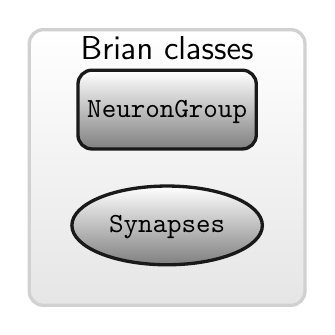
\begin{tikzpicture} [rounded corners=5pt,
	   neurongroup/.style 2 args = {rectangle, minimum size=#1, 
	                                very thick, draw=#2!80!black!90, top color=white,
                                    bottom color=#2!80!black!50,
                                    font=\ttfamily, text height=1.5ex,text depth=.25ex},
       synapsegroup/.style 2 args = {ellipse, minimum size=#1, 
	                                very thick, draw=#2!80!black!90, top color=white,
                                    bottom color=#2!80!black!50,
                                    font=\ttfamily, text height=1.5ex,text depth=.25ex}]
	%% Neurons
	\node [neurongroup={10mm}{black}] (neu) {NeuronGroup};
	\node [synapsegroup={10mm}{black},below=9.5mm of neu.center] (syn) {Synapses};
	\begin{scope}[on background layer]
		\node [neurongroup={35mm}{white},fit=(neu) (syn),
		       label={[shift={(0ex,-3.5ex)},font=\sffamily]north:{\large Brian classes}}] (classes) {};
	\end{scope}	
\end{tikzpicture}

%----------------------------------------------------------------------------------------------------------------
% Synapse-glia interaction scheme
%----------------------------------------------------------------------------------------------------------------
\begin{tikzpicture} [>=stealth, black!50, text=black, thick,rounded corners=3pt,
	   every new ->/.style = {shorten >=1pt},
	   every node/.style={font=\footnotesize},
	   neurongroup/.style 2 args = {rectangle, minimum size=#1, 
	                                very thick, draw=#2!80!black!90, top color=white,
                                    bottom color=#2!80!black!50,
                                    font=\ttfamily, text height=1.5ex,text depth=.25ex},
       synapsegroup/.style 2 args = {ellipse, minimum size=#1, 
	                                very thick, draw=#2!80!black!90, top color=white,
                                    bottom color=#2!80!black!50,
                                    font=\ttfamily, text height=1.5ex,text depth=.25ex}]
	%% Neurons
	\node [neurongroup={10mm}{Purple}] (input) {source\_neurons};
	\node [neurongroup={10mm}{Purple},below=8.5mm of exc.center] (output) {target\_neurons};
		
	%% Synapses
	\node [synapsegroup={8mm}{Purple}, below right= -3pt and 2.5cm of exc.south] (syn) {synapses};
	
	%% Extracellular space
	\node [synapsegroup={8mm}{Lime},right = 3.75cm of input.east] (ecs_s2a) {ecs\_syn\_to\_astro};
	\node [synapsegroup={8mm}{Magenta},right = 3.75cm of output.east] (ecs_a2s) {ecs\_astro\_to\_syn};

	%% Astrocytes
	\node [neurongroup={20mm}{DarkGreen},right = 6.6cm of syn.east,
	       label={[shift={(0ex,2.5ex)},text height=1.5ex,text depth=.25ex,align=center]center:{\normalsize\texttt{astrocyte}}}] (astro) {};
	\node [below=-0.75ex,align=center] at (astro.center) {with\\gliotransmitter\\release};

	%% Paths
	\draw[->] let \p1=(syn.north) in (input.east) -| (\x1-2mm,\y1)
	          node[above,align=center,near start] {spike event};
	\draw[->] let \p1=(syn.south) in (\x1-2mm,\y1) |- (output.east);
	\draw[->,Lime,text=black] let \p1=(syn.north) in (\x1+2mm,\y1) |- (ecs_s2a.west)
	          node[above,align=center,near end] {\texttt{Y\_S}};
	\draw[->,Magenta,text=black] let \p1=(syn.south) in (ecs_a2s.west) -| (\x1+2mm,\y1) 
	          node[below,align=center,near start] {\texttt{G\_A (summed)}};
	\draw[->,Lime,text=black] let \p1=(ecs_s2a.east), \p2=(astro.west) in (\p1) -- (\x2,\y1) 
	          node[above,align=center,midway] {\texttt{Y\_S (summed)}};
	\draw[->,Magenta,text=black] let \p1=(astro.west), \p2=(ecs_a2s.east) in (\x1,\y2) -- (\p2) 
	          node[below,align=center,midway] {\texttt{G\_A}};	          
\end{tikzpicture}

%----------------------------------------------------------------------------------------------------------------
% Gliotransmission scheme (w/ external stimulation of astrocytes)
%----------------------------------------------------------------------------------------------------------------
\begin{tikzpicture} [>=stealth, black!50, text=black, thick,rounded corners=3pt,
	   every new ->/.style = {shorten >=1pt},
	   every node/.style={font=\footnotesize},
	   neurongroup/.style 2 args = {rectangle, minimum size=#1, 
	                                very thick, draw=#2!80!black!90, top color=white,
                                    bottom color=#2!80!black!50,
                                    font=\ttfamily, text height=1.5ex,text depth=.25ex},
       synapsegroup/.style 2 args = {ellipse, minimum size=#1, 
	                                very thick, draw=#2!80!black!90, top color=white,
                                    bottom color=#2!80!black!50,
                                    font=\ttfamily, text height=1.5ex,text depth=.25ex}]
	%% Neurons
	\node [neurongroup={10mm}{Purple}] (input) {source\_neurons};
	\node [neurongroup={10mm}{Purple},below=8.5mm of exc.center] (output) {target\_neurons};
		
	%% Synapses
	\node [synapsegroup={8mm}{Purple}, below right= -3pt and 2.5cm of exc.south] (syn) {synapses};
	
	%% Extracellular space
	\node [synapsegroup={8mm}{Magenta},right = 3.75cm of output.east] (ecs_a2s) {ecs\_astro\_to\_syn};

	%% Astrocytes
	\node [neurongroup={20mm}{DarkGreen},right = 6.6cm of syn.east,
	       label={[shift={(0ex,2.5ex)},text height=1.5ex,text depth=.25ex,align=center]center:{\normalsize\texttt{astrocyte}}}] (astro) {};
	\node [below=-0.75ex,align=center] at (astro.center) {with\\gliotransmitter\\release};

	%% Paths
	\draw[->] let \p1=(syn.north) in (input.east) -| (\x1-2mm,\y1)
	          node[above,align=center,near start] {spike event};
	\draw[->] let \p1=(syn.south) in (\x1-2mm,\y1) |- (output.east);
	\draw[->,Magenta,text=black] let \p1=(syn.south) in (ecs_a2s.west) -| (\x1+2mm,\y1) 
	          node[below,align=center,near start] {\texttt{G\_A (summed)}};
	\draw[->,Lime,text=black] let \p1=(input.west), \p2=(astro.west), \p3=(ecs_a2s.east) in (\x3,\y1) -- (\x2,\y1) 
	          node[above,align=center,midway] {\texttt{Y\_S}}
	          node[below,align=left,midway] {external\\stimulation};
	\draw[->,Magenta,text=black] let \p1=(astro.west), \p2=(ecs_a2s.east) in (\x1,\y2) -- (\p2) 
	          node[below,align=center,midway] {\texttt{G\_A}}
	          node[below=2.0ex,align=left,midway] {gliotransmitter in the\\extracellular space};      
\end{tikzpicture}

%----------------------------------------------------------------------------------------------------------------
% Astrocyte networks (gap junctions) (old version w/ astrocyte stimulation by synaptic input)
%----------------------------------------------------------------------------------------------------------------
\begin{tikzpicture} [>=stealth, black!50, text=black, thick,rounded corners=3pt,
	   every new ->/.style = {shorten >=1pt},
	   every node/.style={font=\footnotesize},
	   neurongroup/.style 2 args = {rectangle, minimum size=#1, 
	                                very thick, draw=#2!80!black!90, top color=white,
                                    bottom color=#2!80!black!50,
                                    font=\ttfamily, text height=1.5ex,text depth=.25ex},
       synapsegroup/.style 2 args = {ellipse, minimum size=#1, 
	                                very thick, draw=#2!80!black!90, top color=white,
                                    bottom color=#2!80!black!50,
                                    font=\ttfamily, text height=1.5ex,text depth=.25ex}]
	%% Neurons
	\node [neurongroup={10mm}{Purple}] (input) {source\_neurons};
	\node [neurongroup={10mm}{Purple},below=8.5mm of exc.center] (output) {target\_neurons};
		
	%% Synapses
	\node [synapsegroup={8mm}{Purple}, below right= -3pt and 2.5cm of exc.south] (syn) {synapses};
	
	%% Extracellular space
	\node [synapsegroup={8mm}{Lime},right = 0.5cm of syn.east] (ecs_s2a) {ecs\_syn\_to\_astro};

	%% Reference node
	\node [draw=none] (start) {};	

	%% Astrocytes
	\node [neurongroup={20mm}{DarkGreen},right = 6.6cm of syn.east] (astro) {astrocytes};

	%% Gap junctions
	\node [synapsegroup={8mm}{DarkGreen},right = 0.25cm of astro.east] (gjc) {astro\_to\_astro};

	%% Paths
	\draw[->] (input.east) -| (syn.north)
	          node[above,align=center,near start] {spike event};
	\draw[->] (syn.south) |- (output.east);
	\draw[->,Lime,text=black] (syn.east) -- (ecs_s2a.west)
	          node[above,align=center,midway] {\texttt{Y\_S}};
	\draw[->,Lime,text=black] let \p1=(ecs_s2a.east), \p2=(astro.west) in (\p1) -- (\x2,\y1) 
	          node[above,align=center,midway] {\texttt{Y\_S (summed)}};
	\draw[->,DarkGreen,text=black] let \p1=(astro.east) in (\x1,\y1 + 8mm) -| (gjc.north) 
	          node[above,align=center,near start] {\texttt{I\_coupling}}
	          node[above=0.6ex,align=left] at (gjc.north east) {IP$_3$ diffusion by\\gap junctions};
	\draw[->,DarkGreen,text=black] let \p1=(astro.east) in (gjc.south) |- (\x1,\y1 - 8mm)
	          node[below,align=center,near end] {\texttt{I\_coupling}};	          
\end{tikzpicture}

%----------------------------------------------------------------------------------------------------------------
% Astrocyte networks (gap junctions)
%----------------------------------------------------------------------------------------------------------------
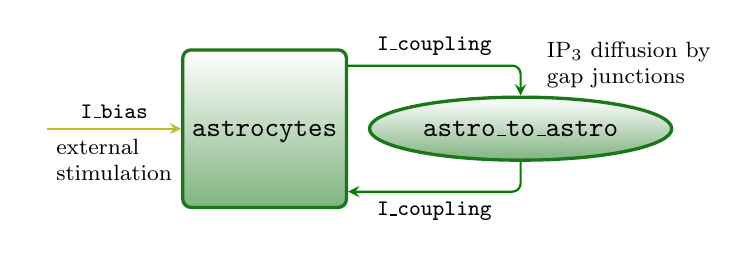
\begin{tikzpicture} [>=stealth, black!50, text=black, thick,rounded corners=3pt,
	   every new ->/.style = {shorten >=1pt},
	   every node/.style={font=\footnotesize},
	   neurongroup/.style 2 args = {rectangle, minimum size=#1, 
	                                very thick, draw=#2!80!black!90, top color=white,
                                    bottom color=#2!80!black!50,
                                    font=\ttfamily, text height=1.5ex,text depth=.25ex},
       synapsegroup/.style 2 args = {ellipse, minimum size=#1, 
	                                very thick, draw=#2!80!black!90, top color=white,
                                    bottom color=#2!80!black!50,
                                    font=\ttfamily, text height=1.5ex,text depth=.25ex}]
	%% Reference node
	\node [draw=none] (start) {};	

	%% Astrocytes
	\node [neurongroup={20mm}{DarkGreen},right = 1.7cm of start.east] (astro) {astrocytes};

	%% Gap junctions
	\node [synapsegroup={8mm}{DarkGreen},right = 0.25cm of astro.east] (gjc) {astro\_to\_astro};

	%% Paths
	\draw[->,Lime,text=black] (start) -- (astro.west) 
	          node[above,align=center,midway] {\texttt{I\_bias}}
	          node[below,align=left,midway] {external\\stimulation};
	\draw[->,DarkGreen,text=black] let \p1=(astro.east) in (\x1,\y1 + 8mm) -| (gjc.north) 
	          node[above,align=center,near start] {\texttt{I\_coupling}}
	          node[above=0.6ex,align=left] at (gjc.north east) {IP$_3$ diffusion by\\gap junctions};
	\draw[->,DarkGreen,text=black] let \p1=(astro.east) in (gjc.south) |- (\x1,\y1 - 8mm)
	          node[below,align=center,near end] {\texttt{I\_coupling}};	          
\end{tikzpicture}

%----------------------------------------------------------------------------------------------------------------
% Astrocyte activation by synaptic inputs
%----------------------------------------------------------------------------------------------------------------
\begin{tikzpicture} [>=stealth, black!50, text=black, thick,rounded corners=3pt,
	   every new ->/.style = {shorten >=1pt},
	   every node/.style={font=\footnotesize},
	   neurongroup/.style 2 args = {rectangle, minimum size=#1, 
	                                very thick, draw=#2!80!black!90, top color=white,
                                    bottom color=#2!80!black!50,
                                    font=\ttfamily, text height=1.5ex,text depth=.25ex},
       synapsegroup/.style 2 args = {ellipse, minimum size=#1, 
	                                very thick, draw=#2!80!black!90, top color=white,
                                    bottom color=#2!80!black!50,
                                    font=\ttfamily, text height=1.5ex,text depth=.25ex}]
	%% Neurons
	\node [neurongroup={10mm}{Purple}] (input) {source\_neurons};
	\node [neurongroup={10mm}{Purple},below=8.5mm of exc.center] (output) {target\_neurons};
		
	%% Synapses
	\node [synapsegroup={8mm}{Purple}, below right= -3pt and 2.5cm of exc.south] (syn) {synapses};
	
	%% Extracellular space
	\node [synapsegroup={8mm}{Lime},right = 0.5cm of syn.east] (ecs_s2a) {ecs\_syn\_to\_astro};

	%% Astrocytes
	\node [neurongroup={20mm}{DarkGreen},right = 6.6cm of syn.east] (astro) {astrocyte};

	%% Paths
	\draw[->] (input.east) -| (syn.north)
	          node[above,align=center,near start] {spike event};
	\draw[->] (syn.south) |- (output.east);
	\draw[->,Lime,text=black] (syn.east) -- (ecs_s2a.west)
	          node[above,align=center,midway] (ys) {\texttt{Y\_S}}
	          node[below=1cm,align=left,anchor=west] at (ys.west) {neurotransmitter in the\\extrasynaptic space};
	\draw[->,Lime,text=black] let \p1=(ecs_s2a.east), \p2=(astro.west) in (\p1) -- (\x2,\y1) 
	          node[above,align=center,midway] {\texttt{Y\_S (summed)}};
\end{tikzpicture}

%----------------------------------------------------------------------------------------------------------------
% Astrocyte ring scheme
%----------------------------------------------------------------------------------------------------------------
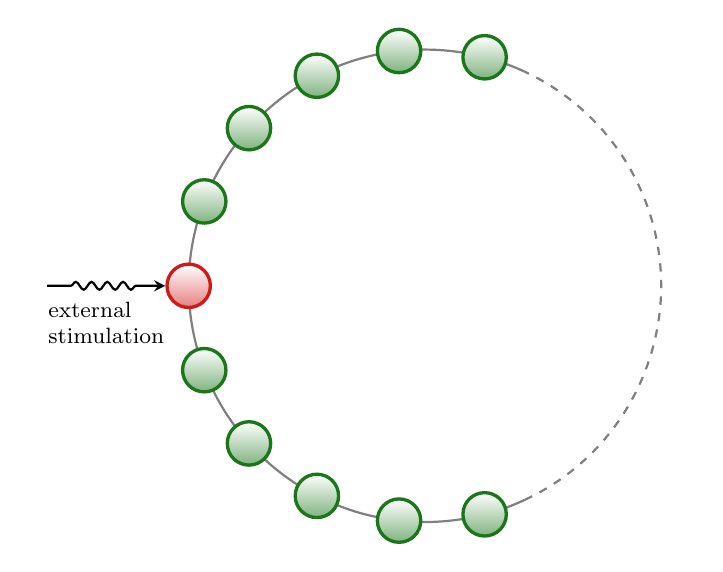
\begin{tikzpicture} [scale=3,
       >=stealth, black!50, text=black, thick,rounded corners=3pt,
	   every new ->/.style = {shorten >=1pt},
	   every node/.style={font=\footnotesize},
	   astrogroup/.style 2 args = {circle, minimum size=#1, 
	                                very thick, draw=#2!80!black!90, top color=white,
                                    bottom color=#2!80!black!50,
                                    font=\ttfamily, text height=1.5ex,text depth=.25ex}]
                                    
	%% First draw the ring as three arches
	\draw (0,0) arc [start angle=180,delta angle=115,x radius=1,y radius=1]
		node[pos=0] (origin) {}
		node[pos=1] (topend) {}
		\foreach [count=\i] \p in {0.182,0.364,...,0.91}
			{node[pos=\p] (tn\i) {}};
	\draw[dashed] (topend) arc [start angle=245,end angle=115,x radius=-1,y radius=1]
	        node[pos=1] (botend) {};
	\draw (origin) arc [start angle=180,delta angle=-115,x radius=1,y radius=1]
		\foreach [count=\i] \p in {0.182,0.364,...,0.91}
			{node[pos=\p] (bn\i) {}};	
	
	%% Add astrocytic nodes (using previously-defined locations)
	\node [astrogroup={5mm}{red}] (input) at (origin) {};
    \foreach [count=\i] \p in {0.182,0.364,...,0.91}
    	{\node [astrogroup={5mm}{DarkGreen}] at (tn\i) {};
    	 \node [astrogroup={5mm}{DarkGreen}] at (bn\i) {};}
    
	%% Add input stimulus
	\node[left=1.5cm of input.west] (in) {};
	\draw[->,black,rounded corners=0cm,text=black,decorate,
	      decoration={snake,amplitude=.5mm,segment length=2mm,
	                  pre length=3mm,post length=3mm}] (in) -- (input.west)
	      node[below=.5ex,align=left,midway] {external\\stimulation};        
\end{tikzpicture}
\end{document}


